%!TEX root = ../dissertation.tex
\chapter{Definitions}\label{ch:definitions}
\newthought{We present definitions and explanations} of concepts and terms that are used throughout this work. 
Throughout this chapter, we provide examples from a hypothetical dataset, Computer.
We will use Computer to answer the problem of predicting whether someone uses a Mac or a PC.
Computer is a dataset comprised of $20$ individuals, whether they use a Mac or PC, and other personal details that may help with the prediction.

\section{Rules}

\begin{figure}[t!]
%\vspace{-3mm}
\begin{algorithmic}
\normalsize
\State {\normalfont Rule 1}: \bif $age < 25$ \bthen $Mac$\,

\begin{raggedleft}
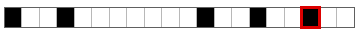
\includegraphics[width=0.5\textwidth]{figs/rule_1_cap.png}
\end{raggedleft}
\State {\normalfont Rule 2}: \bif $(education=college)$ \bthen $Mac$\,

\begin{raggedleft}
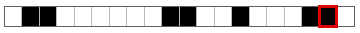
\includegraphics[width=0.5\textwidth]{figs/rule_2_cap.png}
\end{raggedleft}
\State {\normalfont Rule 3}: \bif $age > 45 \wedge \neg (job=software\text{ }engineer)$ \bthen $PC$\,

\begin{raggedleft}
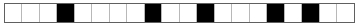
\includegraphics[width=0.5\textwidth]{figs/rule_3_cap.png}
\end{raggedleft}
\State {\normalfont Rule 4}: \bif $\neg (residence=california)$ \bthen $PC$\,

\begin{raggedleft}
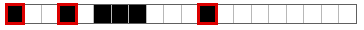
\includegraphics[width=0.5\textwidth]{figs/rule_4_cap.png}
\end{raggedleft}
\end{algorithmic}
%\vspace{-3mm}
\caption{Example rules from the Computer dataset .
The bit vector below the rule is a visual representation of the rule---each box is a data point.
Black boxes represent data points that are classified by a rule.
Data points that are classified incorrectly are outlined in red.
}
\label{fig:rules}
\end{figure}

A \textit{rule} is an \emph{if-then} statement consisting of a boolean antecedent and a classification label.
We are working in the realm of binary classification, so the label is either a $0$ or a $1$ (or an equivalent label).
The boolean antecedents are generated from the rule mining mechanism of Letham et al.~\cite{LethamRuMcMa15} and are a conjunction of boolean features.
These antecedents are \textit{satisfied} by some data points (also called \textit{samples}) and not for others.
We say a rule \textit{classifies} a given data point when the antecedent is satisfied for that data point.
A rule's \textit{support} is comprised of all of the data points that are classified by a rule.
Rules therefore have an inherent accuracy based on their support.
Fig \ref{fig:rules} provides an example of $4$ rules that could be mined from the Computer dataset.
Rule 1, has a support of $5$ but only classifies $4$ of those samples correctly---thus its inherent accuracy is $80$\%.

\section{Rule Lists}

\begin{figure}[t!]
%\vspace{-3mm}
\begin{algorithmic}
\normalsize

\State \textbf{Rule List 1}
\State \bif $age < 25$ \bthen $Mac$\,
\State \belif $\neg (residence=california)$ \bthen $PC$\,
\State \belse $PC$

\begin{raggedleft}
\vspace{1mm}
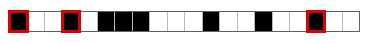
\includegraphics[width=0.7\textwidth]{figs/rule_list_1_cap.png}
\end{raggedleft}
\State \textbf{Rule List 2}
\State \bif $\neg (residence=california)$ \bthen $PC$\,
\State \belif $age < 25$ \bthen $Mac$\,
\State \belse $PC$

\begin{raggedleft}
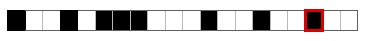
\includegraphics[width=0.7\textwidth]{figs/rule_list_2_cap.png}
\end{raggedleft}

\end{algorithmic}
%\vspace{-3mm}
\caption{Example rule lists from the Computer dataset made using Rule 1, Rule 4, and a default rule.
As in Fig \ref{fig:rules}, black boxes represent data points captured by the rules in the rule list and red marks incorrect classification.
All of the white boxes are classified by the default rule.
Rule 4 has an accuracy of 50\% in Rule List 2, but an accuracy of 100\% in Rule List 1 when it comes after Rule 1.
Thus, despite the two rule lists being permutations of each other, Rule List 1 performs much better than Rule List 2.}
\label{fig:rule-list-computer}
\end{figure}

%Let us define a training dataset of size N as $\{x_n, y_n\}_{n=1}^N$ where each $x_n \in \{0, 1\}^J$ are binary features and each $y_n \in \{0, 1\}$ are binary labels.
%Each rule $x_n$ therefore classifies some of the data points (those indices where $x_{n, j} = 1$).
%Define a rulelist $\mathbf{r} = (r_1, r_2, ... , r_k, r_0)$ where each $r_i \in \{x_n\}_{n=1}^N, \forall i > 0$.
%$r_0$ is defined as the default rule, which makes a prediction on all data points that are not captured in rules $1 ... k$. 
A \textit{rule list} is an ordered collection of rules.
As defined above, rules have an inherent accuracy based on what data they classify and how they predict the label.
As we combine these rules into rule lists, however, only the first rule that classifies any given data point can make a prediction for that data point.
Thus, we say a rule \textit{captures} a given data point if it is the first rule in a rule list to classify that data point.
Therefore, when rules are placed into a rule list, their accuracy is based on what data they capture---which is not necessarily the same as what data they classify.
They can perform better or worse than their inherent accuracy depending on what rules come before them in a given rule list.
For example, we can see in Fig \ref{fig:rule-list-computer} that even though Rule 4 only has an inherent accuracy of 50\%, in Rule List 1 it has an accuracy of 100\% because it is placed below Rule 1.

Our algorithm is focused on finding the list that combines rules in an order that maximizes predictive accuracy.
A rule list also has a \textit{default rule}, placed at the end of any rule list, that classifies all data points and predicts the majority label.
This allows a rule list to make predictions for all points because any point not captured by the pre-mined rules is captured by the default rule.
We refer to the length of a rule list as the number of pre-mined rules, without including the default rule.
The rule lists in Fig \ref{fig:rule-list-computer} are both of length 2.
We define a \textit{prefix} as any subset of the rules at the beginning of a rule list.
We will often use prefix to refer to the list of all rules in a rule list except for the default rule.

\section{Objective Function}
Rule lists have a loss function based on the number of points that are misclassified by the rules in the rule list---including misclassifications due to the default rule.
We define our \textit{objective} function to be the sum of that loss and a \textit{regularization term}, which is a constant times the length of the rule list.
This has the effect of preventing overfitting on training datasets as well as discouraging extremely long, and therefore uninterpretable, rule lists.
While the objective is related to accuracy (a higher accuracy means a lower objective), we will be minimizing over the objective function instead of maximizing the accuracy to reap the benefits of the regularization term.
Let RL be a rule list, then:
$$objective(RL) = loss(RL) + \lambda * len(RL)$$
We can calculate the objective for Rule List 1 in Fig \ref{fig:rule-list-computer} as follows.
The loss from rules 1 and 4 is $0.05$, while the loss from the default rule is $0.05$.
Assuming a regularization constant of $\lambda=0.01$, the objective for Rule List  1 is $0.05 + 0.05 + 2 * 0.01 = 0.12$.

\section{Bounds}\label{sec:bounds}
For a set of $n$ rules, there are $n!$ possible rule lists.
Finding the optimal rule list using a brute force approach is infeasible for any problem of reasonable size.
Our algorithm uses the discrete optimization technique of branch-and-bound to solve this combinatorially difficult problem of finding an optimal rule list.
This requires tight bounds that allow us to prune as much of the search space as possible.
These bounds are formalized and proved in Angelino et al.~\cite{AngelinoLaAlSeRu17} and are reproduced in Appendix A.
For clarity, we present informal summaries of the important bounds here.

\subsection{Lower Bound}
We use the term \textit{lower bound} to mean the best possible outcome for the objective function for a given prefix.
We do this by calculating the loss of the prefix and assuming that any points not captured by the prefix will be predicted correctly.
This is equivalent to creating a hypothetical default rule that captures all points perfectly.
Because any future extensions of the prefix can never do better than this perfect default rule, we will be able to use this bound to prune our exploration.
The lower bound also increases monotonically---any rules we add can only make mistakes that this perfect default rule does not make.
Much of the work on CORELS has focused on creating bounds that are as close to the true lower bound as possible.
The smaller the difference between our bounds and the true lower bound, the easier it is to prune sub-optimal rule lists. 
$$lower \text{ } bound(prefix) = loss(prefix) + \lambda * len(prefix)$$
The lower bound for Rule List 1 is therefore $0.05 + 2 * 0.01 = 0.07$, which is less than its objective.
This is due to the fact that the objective function includes the error made by the default rule, but the lower bound has to assume that we could add a rule that would correctly classify the data point that is misclassified by the default rule.

\subsection{Hierarchical Objective Bound}
\begin{figure}[t!]
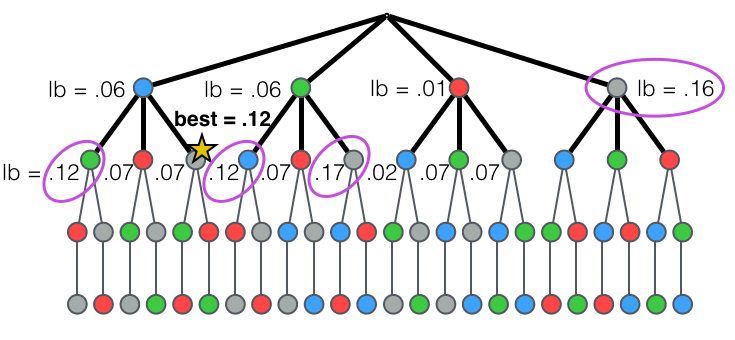
\includegraphics[width=\textwidth]{figs/branch-and-bound-tree.png}
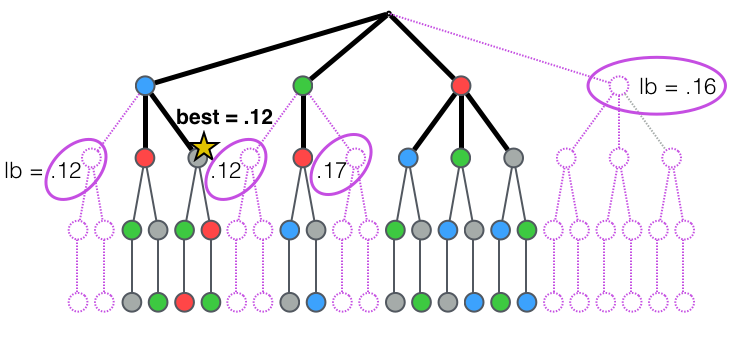
\includegraphics[width=\textwidth]{figs/branch-and-bound-tree-pruned.png}
\caption[Objective bound]{This tree shows the hierarchical objective bound in action.
Each color represents one of our 4 rules from Fig \ref{fig:rules}: blue = Rule 1, green = Rule 2, red = Rule 3, and gray = Rule 4.
Thus, each path in the tree represents a rule list.
Our best objective seen is the rule list (1, 4, default) with an objective of $0.12$.
Any prefixes with lower bound greater than this objective---all prefixes beginning with (4), (1, 2), (2, 1), or (2, 4)---can be pruned and not examined.
The bottom tree shows the pruned prefixes, marked in purple.
\label{fig:objective-bound}}
\end{figure}

The main bound for our algorithm is the \textit{hierarchical objective bound}. 
It says that we do not need to pursue a rule list if it has a lower bound that is worse than the best objective we have already seen.
This follows from the fact that lower bounds increase monotonically, so if the lower bound of Rule List 2 is equal to or worse than the objective of Rule List 1, any extensions of Rule List 2 can never be better than Rule List 1.
This allows us to prune large parts of the search space by not pursuing rule lists that could never be better than something we have already seen.
Fig \ref{fig:objective-bound} provides an example of our pruning mechanism in action.
It shows how an exploration of the search space leads to a difference in the best observed objective and the lower bounds of some rule lists.
Our algorithm will use that difference to prune parts of the search space and reduce a combinatorially large problem into a tractable one.

\subsection{Permutation Bound}
\label{def:perm-bound}

\begin{figure}[t!]
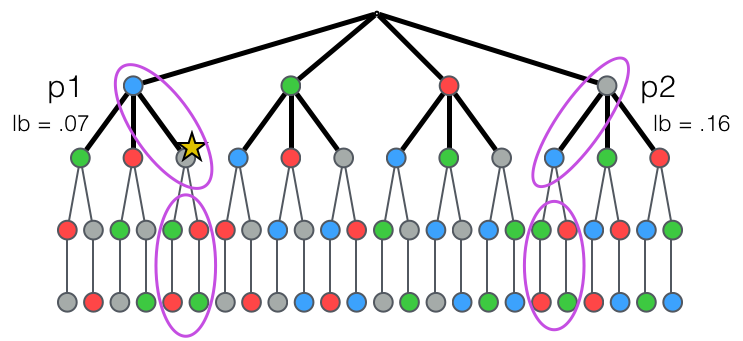
\includegraphics[width=\textwidth]{figs/branch-and-bound-permutations.png}
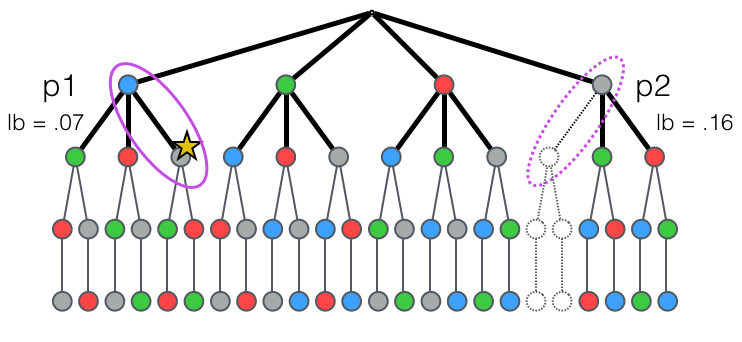
\includegraphics[width=\textwidth]{figs/branch-and-bound-permutations-pruned.png}
\caption[Permutation bound]{This tree shows the use of the permutation bound in action. 
Prefixes (1, 4) and (4, 1) are permutations of each other, so they capture identical data (see Fig \ref{fig:rule-list-computer}).
When we compare their lower bounds, we see the prefix (1, 4) has a better lower bound.
Any rule list beginning with (4, 1) would be worse than the corresponding rule list beginning with (1, 4), so (4, 1) can be pruned and none of its children have to be examined.
\label{fig:permutation-bound}}
\end{figure}

As defined above, every sample is captured by precisely one rule---in the prefix (1, 4), any sample that is captured by rule 1 cannot be captured by rule 4. 
Now consider a \textit{permutation} of the prefix (1, 4): the prefix (4, 1).
Any samples that are captured by either rule 1 or 4 but not both will be captured identically in both rule lists.
Samples that are captured by both rules will again be captured the same in both rule lists, though they may be predicted differently in the two rule lists.
Thus, regardless of the order in which the rules appear, prefixes (1, 4) and (4, 1) will capture exactly the same set of data---this can be seen in the bit vectors of Fig \ref{fig:rule-list-computer}.
They will differ only in which rules capture which samples, so their accuracies may differ.
We can use this knowledge to create a bound that we call the \textit{permutation bound}.
If we know that the lower bound of the prefix (1, 4) is better than the lower bound of (4, 1), we can eliminate from consideration all rule lists beginning with (4, 1).
This is due to the fact that any rule list beginning with (1, 4) will capture exactly the same samples as the equivalent rule list beginning with (4, 1), but will have a better objective score.
Fig \ref{fig:permutation-bound} demonstrates the pruning process with the prefixes (1, 4) and (4, 1).
Since (1, 4) has a lower bound of 0.07 while (4, 1) has a lower bound of 0.16, we can prune (4, 1) and not pursue any of its children.

Generalizing this principle allows us to eliminate all but one permutation of a given set of rules.
When we are dealing with these permutations, it is helpful to map all permutations to a single ordering by ordering the rules in numerical order.
We call this the \textit{canonical ordering} of a prefix.
For example, the prefixes (1, 4) and (4, 1) both map to the canonical ordering (1, 4).

\subsection{Support Bounds}
Due to the regularization term in our objective function, adding a rule that does little to improve accuracy will harm the overall objective score.
This allows us to place bounds that rely on the support of the rules we add.
It never makes sense to add a rule that increases the objective function, so we consider adding only those rules that capture sufficiently many points correctly to overcome the regularization penalty.
By definition, rules that do not capture enough of the remaining points cannot capture them correctly, so this provides us with two closely related bounds.
As our rule lists grow, many rules do not capture enough points and this bound begins to play a larger role.

\subsection{Equivalent Points Bound}
This bound relies on the similarities within the structure of our dataset.
In our dataset, we may encounter two data points that have the same features but different labels.
We call the set of these data points \textit{equivalence points} and describe the label that occurs less often as the \textit{minority} label.
Since equivalence points have identical features, any rule that classifies one point in an equivalence class will also classify all other points in that class.
However, it is impossible to correctly predict equivalence points with different labels using a single rule.
So, for a given class of equivalence points, we know that we will mispredict all of the points with a minority label.
We can thus update our lower bound to be tighter than just assuming that the default rule will capture all remaining points correctly.
Now, we assume that any remaining points with a minority label will be captured incorrectly.
This gives us much tighter lower bounds and, in practice, allows us to prune more efficiently.

In our Computer dataset, for instance, we might have 3 people who are in college and form an equivalence class.
Now, 2 of those people use Macs and will be correctly classified by Rule 1.
However, we will never correctly classify that 3rd person who uses a PC because any rule will always predict Mac to maximizes its accuracy.
So, our lower bound should take into account the fact that we will always mispredict that person.

\section{Curiosity}
\label{def:curiosity}
There are a number of different ways to explore the search space (see Section \ref{sec:queue}).
Some methods, such as BFS, prioritize exploration---looking at all rule lists of a given length before proceeding to the next length.
Others, such as ordering by lower bound, focus purely on exploiting the best prefixes that we have seen.
We define a new metric, \textit{curiosity}, that combines exploration and exploitation.
Lower values of curiosity mark prefixes that we explore first.
Curiosity is a function of both the lower bound and the number of samples captured.
This prioritizes rule lists that still have many samples left to capture (exploration) while also pursuing rule lists with promising lower bounds (exploitation).
$$curiosity(RL) = (lowerBound(RL) - minority)  * (nsamples / |captured(RL)|)$$
Assuming a minority value of 0, we can see that the curiosity of Rule List 1 is $(.07 - 0) * (20 / 8) = 0.175$, while the curiosity of Rule List 2 is $(.22 - 0) * (20 / 8) = 0.55$.
Thus, curiosity prioritizes extending the more promising rule list.

\section{Remaining Search Space}
One metric for tracking the efficacy of our optimizations will be observing how quickly we reduce the remaining search space.
We start with a combinatorially large search space, but quickly reduce it using our bounds.
We calculate the remaining search space by determining how much each prefix could be expanded.
We do this for every prefix we have evaluated and not eliminated.
Due to our regularization term, we are able to bound the maximum length of any optimal rule list as our best objective gets updated.
This upper bound on the maximum length of an optimal rule list allows us to place an upper bound on the remaining search space as well.
The search space of our problem can be visualized as a tree with fanout $n$--depth.
From the root, there are $n$ rules we can add, and then we can add $n - 1$ rules to each of those rules, and so forth.
However, as the best objective we have seen gets better, there are more paths of the tree that we can eliminate and so our search tree grows smaller.
%We find that the remaining search space decreases rapidly at the beginning of execution, then slowly decreases until the very end of execution when it again rapidly decreases.

\section{Datasets}
\label{def:datasets}
All of our datasets are split into a training set and a test dataset to test for accuracy.
We then divide the dataset 90-10 for training and test sets.
In addition, we split our training and test sets into 10 folds to perform cross validation.
For our analysis that does not involve accuracy calculations, our performance numbers come from running on a single fold.

The COMPAS dataset is a list of criminal offenders and information about them and their records.
The classification problem that we're trying to solve is whether or not a given offender will commit another crime within 2 year of being arrested.
As mentioned in the introduction, this problem is currently being handled through the use of a black box model because the authors of that model claim that adding interpretability would harm accuracy.
This black box model has been accused of racially biased predictions~\cite{LarsonMaKiAn16}.
We explore this dataset with the goal of providing an interpretable, non-biased model that has accuracy comparable to state of the art black-box models.

The COMPAS dataset has 7214 individuals, meaning our training set has 6489 data points.
2947 (45.1\%) of these individuals are labeled "yes", meaning they have committed a second crime after being arrested---while the other 3542 (54.9\%) individuals are labeled "no".
On this particular dataset, COMPAS scores achieve 61\% accuracy for predicting recidivism. 
The creator of the COMPAS score, Tim Brennan, has previously shown an AUC of .68 for predicting any offense on a smaller dataset of 2300 individuals~\cite{BrennanDiEh09}.
He also claims that it's difficult to get good accuracy without using racially influenced features, saying:
\begin{quote}
``it is difficult to construct a score that does not include items that can be correlated with race such as poverty, joblessness and social marginalization. `If those are omitted from your risk assessment, accuracy goes down',€™~[Brennan] said.''~\cite{LarsonMaKiAn16}
\end{quote}
\noindent We are able to extract 155 rules from the dataset, including rules that involve the race of the individual.

The Stop and Frisk dataset is a list of stops made by the New York City Police Department (NYPD) that contains information about the outcome of that stop: whether an individual was frisked, searched, or found carrying a weapon.
The classification problem that we are trying to solve are whether someone is carrying a weapon when stopped (which we refer to from now on as Weapon).
Stop and Frisk has been a controversial program and recent work has alleged that blacks and Hispanics are disproportionately stopped~\cite{GoelRaSh16}.
The authors of that work further suggest that it would be ideal to provide police officers with a simple heuristic about whether or not to make a stop.
We hope to provide a model that is short and easy to remember, but also has high predictive accuracy when it comes to finding weapons or other contraband.

This dataset is composed of 45787 individuals of whom 3.3\% are carrying a weapon.
We are able to extract 46 rules, some of which include features involving the race of the individual.
